%  \documentclass[DIV=12, a4]{scrartcl}
%\documentclass[12pt, a5]{scrartcl}
\documentclass[a4]{scrreprt}

\usepackage[
fancytheorems, 
noindent, 
%spacingfix, 
%noheader
]{adam}

% \documentclass[a4paper]{report}
% \usepackage[
% % fancytheorems, 
% noindent, 
% %spacingfix, 
% %noheader
% ]{vanilla}

\usepackage{tikz}
\usepackage{enumitem}

% \usepackage{subfig}

\setcounter{chapter}{-1}

\title{Vectors and Matrices}
% \subtitle{Adam Kelly}
\author{Adam Kelly}
\date{\today}

% \title{Vectors and Matirces}
% % \subtitle{Adam Kelly}
% \author{Adam Kelly, Lectured by Dr. J. Evans}
% \date{Michaelmas 2020}

\begin{document}

\maketitle

\begin{abstract}
	% \vspace{2\baselineskip}
	% {\color{red} None of the notes here have been reviewed at all, and are just exactly what was taken down live in the lectures. I would turn around now and come back in a few days, when I have gone back, cleaned things up, fixed explanations and added some structure.}
	% \vspace{5\baselineskip}

	This set of notes is a work-in-progress account of the course `Vectors and Matrices', originally lectured by Dr. Jonathan Evans in Michaelmas 2020 at Cambridge. These notes are not a transcription of the lectures, but they do roughly follow what was lectured (in content and in structure).

	These notes are my own view of what was taught, and should be somewhat of a superset of what was actually taught. I frequently provide different explanations, proofs, examples, and so on in areas where I feel they are helpful. Because of this, this work is likely to contain errors, which you may assume are my own. If you spot any or have any other feedback, I can be contacted at \href{mailto:ak2316@cam.ac.uk}{ak2316@cam.ac.uk}.

	% During the creation of this document, I consulted a number of other books and resources. All of these are listed in the bibliography. 
\end{abstract}

\tableofcontents

\clearpage

\chapter{Introduction}

Vectors and Matrices covers topics in both algebra and geometry, and the way in which they relate to one another. The course uses approaches that are quite varied in their nature (can be abstract or more concrete, conceptual or more computational, and so on). You will need to be able to fluently switch between these approaches.

The course assumes that you are vaguely familiar with Euclidean and coordinate geometry, along with the idea of geometric transformations.

\section{Course Structure}

This course is divided into a number of chapters.

\begin{enumerate}
	\item \emph{Complex Numbers}

	This chapter takes the point of view of thinking of points in the plane as pairs of real numbers, and defining `multiplication' on it to turn it into the complex numbers.

	\item \emph{Vectors in Three Dimensions}
	
	Here, we will recap on the relationship between three dimensional vectors and some of theire geometrical applications, and we will discuss things like the dot and cross product. Towards the end of that discussion, we will introduce the `index notation', a powerful and helpful notation for dealing with vectors. We will also introduce the `summation convention', which is also incredibly useful.

	\item \emph{Vectors in a General Setting}
	
	This chapter will discuss what vectors are in general, and different ways of looking at them. We will be particularly concerned with vectors in $\mathbb{R}^n$ and $\mathbb{C}^n$, that is, vectors who's entries are in $\mathbb{R}$ and $\mathbb{C}$ respectively.

	\item \emph{Matrices and Linear Maps}
	
	Picking up on the idea of generalizing vectors, this chapter will consider the idea of a `linear map', an abstraction of matrices. 

	\item \emph{Determinants and Inverses}
	
	This chapter will detail how to define and compute determinants of general $n \times n$ matrices. This will take two points of view, in that we need to be able to compute them but we also must understand what they mean. The relation between determinants and finding inverses of matrices will also be considered.

	\item \emph{Eigenvalues and Eigenvectors}
	
	This chapter also involves both geometry and algebra. The core question of this chapter is: given a linear map or matrix, what does it act on in a very straightforward way?

	\item \emph{Changing Basis, Canonical Forms and Symmetries}
	
	In this final chapter, we will consider a set of far reaching results by trying to describing an arbitrary linear map. These ideas are far reaching, and immensely useful.
\end{enumerate}

\section{Differences to the Lecture Course}

This set of notes may diverge slightly from the lectures. If this occurs, I will attempt to describe the differences in this section.
For now, while these notes are incomplete, I will leave it up to the reader to check themselves what is included or missing.  
% This set of notes differs from what was lectured in a number of areas. I have attempted to briefly outline these changes below.

% In the `Complex Numbers' chapter, I have included a brief section on the historical developments that eventually led to their use today, mainly focusing on the solution to cubic equations.
% This follows the development in Needham's \emph{Visual Complex Analysis}.



\chapter{Complex Numbers}

The complex numbers arose through the study of polynomials, but there is hardly an area of modern mathematics where they are not of use, with applications stretching from number theory to geometry to quantum mechanics.



% \section{Historical Context}

% The complex numbers arose through the study of polynomials, and their serious study really began in the study of the \emph{cubic} polynomials of the form\footnote{This form of a cubic equation is a `depressed', and any general cubic can be expressed in this form.}
% $$
% x^3 - 3px - 2q = 0.
% $$
% The sixteenth century mathematicians del Ferro, Tartaglia and Cardano discovered that this equation could be solved explicitly, with the result being published in Cardano's 1545 work \emph{Ars Magna} (where he mentioned del Ferro as a first author, and noted that Tartaglia had independently found the same result).
% The solution they had obtained was
% $$
% x = \sqrt[3]{q + \sqrt{q^2 - p^3}} + \sqrt[3]{q - \sqrt{q^2 - p^3}}.
% $$
% For example, for the cubic $x^3 - 12x - 20$ we obtain the solution $x = \sqrt[3]{16} + \sqrt[3]{2}$. 

% Some 30 years later, Rafael Bombelli discussed one particular cubic in his work \emph{l'Algebra}. He looked at $x^3 - 15x - 4 = 0$.
% One might observe (through mere trial and error) that $x = 4$ is a solution, but using Cardano's formula, we obtain the solution
% $$
% x = \sqrt[3]{2 + \sqrt{-121}} + \sqrt[3]{2 - \sqrt{-121}}.
% $$
% Indeed, Bombelli noticed this and gave an explanation for how these two solutions were essentially the same, even with the presence of the rather puzzling term $\sqrt{-121}$.
% His explanation essentially began by noting that if we wrote $\sqrt{-121} = 11i$, then we could find that
% \begin{align*}
% 	\sqrt[3]{2 + \sqrt{-121}} &= 2 + ni \\
% 	\sqrt[3]{2 - \sqrt{-121}} &= 2 - ni,
% \end{align*}
% and adding would then result in $2 + ni + 2 - ni = 4$, our other solution.

% Inherent in this explanation was an expectation that this $i$ would obey the many of the same rules of arithmetic that we would expect of, say, a real number. After this work, contributions from mathematicians such as Descartes, Wallis, de Moivre, Euler, Wessel, Argand, Hamilton, Gauss, Cauchy and many others began to build up a rich theory of the \emph{complex numbers}, later developing the field of \emph{complex analysis}, all centered on this construction of some $i$ with the property that $i^2 = -1$. 

% In modern mathematics, complex numbers are used everywhere from number theory to geometry to quantum mechanics.

% \section{Defining the Complex Numbers}

We are going to construct the set of complex numbers, typically denoted by $\C$, from the real numbers $\R$ by adjoining an element $i$ with the property that $i^2 = -1$.

\begin{definition}[Complex Numbers]
	A \vocab{complex number} is a number $z \in \C$ of the form $z = x + yi$ with $x, y \in \R$ such that $i^2 = -1$. 
	
	We call $x = \operatorname{Re}(z)$ is the \vocab{real part}, and $y = \operatorname{Im}(z)$ is the \vocab{imaginary part} of $z$.
\end{definition}

The reals are a subset of the complex numbers, as for $x \in \R$, we have $x + 0i \in \C$. We can do add, subtract, multiply and divide complex numbers in a sensible way, and indeed they form a \emph{field} (we will elaborate on this later).

\begin{definition}[Addition and Subtraction]
	We define \vocab{addition} and \vocab{subtraction} for two complex numbers $z_1 = x_1 + y_1i$ and $z_2 = x_2 + y_2 i$ such that 
	\begin{align*}
		z_1 + z_2 &= (x_1 + x_2) + (y_1 + y_2)i\\
		z_1 - z_2 &= (x_1 - x_2) + (y_1 - y_2)i
	\end{align*}
\end{definition}

% We define the following set of operations on complex numbers.

% \begin{definition}[Arithmetic on Complex Numbers]\label{def:complex-arithmetic}
% 	For $z_1 = x_1 + i y_1$ and $z_2 = x_2 + i y_2$, we define
% \begin{enumerate}[label=(\roman*)]
% 	\item \emph{Addition}. $z_1 + z_2 = (x_1 + x_2) + i(y_1 + y_2)$.
% 	\item \emph{Multiplication}. $z_1 z_2 = (x_1 + i y_1)(x_2 + i y_2) = (x_1 x_2 - y_1 y_2) + i(x_1 y_2 + x_2 y_1)$.
% 	\item \emph{Complex conjugation}. $\overline{z} = z^* = x - iy$.
% 	\item \emph{Modulus}. $r = |z|$ is a non-negative real given by $r^2 = |z|^2 = z \overline{z} = x^2 + y^2$.
% 	\item \emph{Argument}. For nonzero $z$, $\theta = \operatorname{arg}(z)$ is a real defined\footnote{$\operatorname{arg}(z)$ is determined modulo $2\pi$, which follows from $\tan \theta = x/y$.} such that $z = r(\cos \theta + i \sin \theta)$. This is the \vocab{polar form} of $z$.
	
% 	With this we have that
% 	$$
% 	\cos \theta=\frac{x}{\left(x^{2}+y^{2}\right)^{1 / 2}} \quad \quad \sin \theta=\frac{n}{\left(x^{2}+y^{2}\right)^{1 / 2}} \quad \implies  \quad \tan \theta=\frac{y}{x}.
% 	$$

% 	In order for $\theta$ to be unique, we can restrict the range of $\theta$. For example, if $-\pi < \theta \leq \pi$, we call this the \vocab{principle value}. However other choices of range are equally valid.
% \end{enumerate}
% \end{definition}

% \begin{proposition}[Properties of Complex Conjugation]
% 	We have
% 	\begin{enumerate}[label=(\roman*)]
% 		\item $\operatorname{Re}(z) = \frac{1}{2}(z + \overline{z})$.
% 		\item $\operatorname{Im}(z) = \frac{1}{2i}(z - \overline{z})$.
% 		\item $\overline{(\overline{z})} = z$.
% 		\item $\overline{z_1 + z_2} = \overline{z_1} + \overline{z_2}$.
% 		\item $\overline{z_1 z_2} = \overline{z_1} \overline{z_2}$.
% 	\end{enumerate}
% \end{proposition}
% \begin{proof}[Proof Sketch]
% 	A direct check from the definitions.
% \end{proof}


% \begin{definition}[The Argand Diagram/Complex Plane]
% 	Plot $\operatorname{Re}(z)$ and $\operatorname{Im}(z)$ on orthogonal axes, then $r = |z|$ and $\arg(z) = \theta$ are the length and angle as shown.
% 	\begin{center}
		

% \tikzset{every picture/.style={line width=0.75pt}} %set default line width to 0.75pt        

% \begin{tikzpicture}[x=0.75pt,y=0.75pt,yscale=-1,xscale=1]
% %uncomment if require: \path (0,300); %set diagram left start at 0, and has height of 300

% %Shape: Pie [id:dp2413182761278425] 
% \draw  [draw opacity=0][fill={rgb, 255:red, 224; green, 224; blue, 224 }  ,fill opacity=1 ] (182.32,96.76) .. controls (186.1,100.05) and (188.48,104.86) .. (188.49,110.23) -- (170.34,110.24) -- cycle ;
% %Straight Lines [id:da39150586947897015] 
% \draw    (246,24) -- (170.34,110.24) ;
% %Straight Lines [id:da07162620321201185] 
% \draw    (170.34,159.39) -- (170.34,21) ;
% \draw [shift={(170.34,18)}, rotate = 450] [fill={rgb, 255:red, 0; green, 0; blue, 0 }  ][line width=0.08]  [draw opacity=0] (8.93,-4.29) -- (0,0) -- (8.93,4.29) -- cycle    ;
% \draw [shift={(170.34,162.39)}, rotate = 270] [fill={rgb, 255:red, 0; green, 0; blue, 0 }  ][line width=0.08]  [draw opacity=0] (8.93,-4.29) -- (0,0) -- (8.93,4.29) -- cycle    ;
% %Straight Lines [id:da3144480185294898] 
% \draw    (271.68,110.24) -- (110,110.24) ;
% \draw [shift={(107,110.24)}, rotate = 360] [fill={rgb, 255:red, 0; green, 0; blue, 0 }  ][line width=0.08]  [draw opacity=0] (8.93,-4.29) -- (0,0) -- (8.93,4.29) -- cycle    ;
% \draw [shift={(274.68,110.24)}, rotate = 180] [fill={rgb, 255:red, 0; green, 0; blue, 0 }  ][line width=0.08]  [draw opacity=0] (8.93,-4.29) -- (0,0) -- (8.93,4.29) -- cycle    ;
% %Shape: Ellipse [id:dp8293273168033899] 
% \draw  [draw opacity=0][fill={rgb, 255:red, 208; green, 2; blue, 27 }  ,fill opacity=1 ] (242.98,24) .. controls (242.98,22.33) and (244.33,20.98) .. (246,20.98) .. controls (247.67,20.98) and (249.02,22.33) .. (249.02,24) .. controls (249.02,25.67) and (247.67,27.02) .. (246,27.02) .. controls (244.33,27.02) and (242.98,25.67) .. (242.98,24) -- cycle ;

% % Text Node
% \draw (284.89,108.73) node    {$\operatorname{Re}$};
% % Text Node
% \draw (172,172) node    {$\operatorname{Im}$};
% % Text Node
% \draw (263,22) node    {$z$};
% % Text Node
% \draw (193.78,101.93) node  [font=\small]  {$\theta $};
% % Text Node
% \draw (205,57) node  [font=\small]  {$r$};


% \end{tikzpicture}
% 	\end{center}
% \end{definition}

% \begin{example}
% 	For $z = -1 + i \sqrt{3}$, we have $|z| = 2$ and $\arg(z) = \frac{2 \pi}{3} + 2n \pi$ for $n \in \mathbb{Z}$. This is shown on the complex plane below.

% 	\begin{center}
		

% \tikzset{every picture/.style={line width=0.75pt}} %set default line width to 0.75pt        

% \begin{tikzpicture}[x=0.75pt,y=0.75pt,yscale=-1,xscale=1]
% %uncomment if require: \path (0,300); %set diagram left start at 0, and has height of 300

% %Shape: Pie [id:dp2413182761278425] 
% \draw  [draw opacity=0][fill={rgb, 255:red, 224; green, 224; blue, 224 }  ,fill opacity=1 ] (191.75,153.57) .. controls (195.34,151.46) and (199.53,150.25) .. (204,150.25) .. controls (217.25,150.25) and (227.99,160.88) .. (228,173.99) -- (204,174) -- cycle ;
% %Straight Lines [id:da39150586947897015] 
% \draw    (142,70) -- (204,174) ;
% %Straight Lines [id:da07162620321201185] 
% \draw    (204,243) -- (204,21) ;
% \draw [shift={(204,18)}, rotate = 450] [fill={rgb, 255:red, 0; green, 0; blue, 0 }  ][line width=0.08]  [draw opacity=0] (8.93,-4.29) -- (0,0) -- (8.93,4.29) -- cycle    ;
% \draw [shift={(204,246)}, rotate = 270] [fill={rgb, 255:red, 0; green, 0; blue, 0 }  ][line width=0.08]  [draw opacity=0] (8.93,-4.29) -- (0,0) -- (8.93,4.29) -- cycle    ;
% %Straight Lines [id:da3144480185294898] 
% \draw    (339,174) -- (69,174) ;
% \draw [shift={(66,174)}, rotate = 360] [fill={rgb, 255:red, 0; green, 0; blue, 0 }  ][line width=0.08]  [draw opacity=0] (8.93,-4.29) -- (0,0) -- (8.93,4.29) -- cycle    ;
% \draw [shift={(342,174)}, rotate = 180] [fill={rgb, 255:red, 0; green, 0; blue, 0 }  ][line width=0.08]  [draw opacity=0] (8.93,-4.29) -- (0,0) -- (8.93,4.29) -- cycle    ;
% %Shape: Ellipse [id:dp8293273168033899] 
% \draw  [draw opacity=0][fill={rgb, 255:red, 208; green, 2; blue, 27 }  ,fill opacity=1 ] (138,70) .. controls (138,67.79) and (139.79,66) .. (142,66) .. controls (144.21,66) and (146,67.79) .. (146,70) .. controls (146,72.21) and (144.21,74) .. (142,74) .. controls (139.79,74) and (138,72.21) .. (138,70) -- cycle ;

% % Text Node
% \draw (355.5,172) node    {$\operatorname{Re}$};
% % Text Node
% \draw (206,254) node    {$\operatorname{Im}$};
% % Text Node
% \draw (108.5,47) node    {$-1+i\sqrt{3}$};
% % Text Node
% \draw (140,128) node  [font=\small]  {$|z|=2$};
% % Text Node
% \draw (257,140) node  [font=\small]  {$\operatorname{Arg}( z) =\frac{2\pi }{3}$};


% \end{tikzpicture}
% 	\end{center}

% 	Note that $\tan \theta = - \sqrt{3}$, so $\theta = \frac{2 \pi}{3} + 2n \pi$, or $\theta = -\frac{\pi}{3} + 2n \pi$, which is $\arg(-z)$. This is notable because it is common to write $\arg(z) = \arctan(y/x)$, but that is not quite correct.
% \end{example}


% \section{Basic Properties of Complex Numbers}

% In this section, we will consider the consequences of the definitions given in the previous section.
% Let us begin by defining the notion of a field.

% \begin{definition}
% 	A \vocab{field} is a thing yeah.
% \end{definition}

% \begin{proposition}
% 	$\mathbb{C}$ with addition and multiplication is a field.
% \end{proposition}
% \begin{proof}
% 	Fill in details here.
% \end{proof}

% The next consequence is the `Fundamental Theorem of Algebra'.
% This is something that's important to know about, but we will not prove it.

% \begin{theorem}[Fundamental Theorem of Alegbra]
% 	A polynomial $p(z)$ of degree $n$ with coefficients in $\mathbb{C}$ can be written as a product of $n$ linear factors. That is, if we have a polynomial
% 	$$
% 	p(z) = c_n z^n + c_{n - 1} z^{n - 1} + \cdots + c_1 z + c_0
% 	$$
% 	with $c_i \in \mathbb{C}$ and $c_n \neq 0$, then we can write
% 	$$
% 	p(z) = (z - \alpha_1) (z - \alpha_2) \cdots (z - \alpha_n),
% 	$$ 
% 	for some $\alpha_i \in \mathbb{C}$ not necissarily distinct.
% \end{theorem}
% \begin{proof}[Proof Omitted]
% 	See the IB course `Complex Methods/Analysis'.
% \end{proof}

% {\color{red} TODO: fill in on-paper notes.}

% \section{Exponential and Trigonometric Functions}

% We define the functions $\exp$, $\cos$ and $\sin$ on the complex numbers by
% \begin{align*}
% 	\exp(z) &= e^z = \sum_{n = 0}^\infty \frac{1}{n!} z^n \\
% 	\cos (z) &= \frac{1}{2}(e^{iz} + e^{-iz}) = 1 - \frac{1}{2!} z^2 + \frac{1}{4!} z^4 + \cdots \\
% 	\sin (z) &= \frac{1}{2i}(e^{iz} - e^{-iz}) = z - \frac{1}{3!}z^3 + \frac{1}{5!} z^5 + \cdots.
% \end{align*}
% These series converge for all $z \in \C$ (this is discussed rigorously in the course `Analysis I').

% \begin{proposition}
% 	For all $z, w \in \C$, we have $e^z e^w = e^{z + w}.$
% \end{proposition}
% \begin{proof}[Proof]
% 	Multiplying the series on the left, we consider the terms of degree $n$:
% 	$$
% 	\sum_{r=0}^{n} \frac{1}{r !} z^{r} \frac{1}{(n-r) !} w^{n-r}=\frac{1}{n !}(z+w)^{n},
% 	$$
% 	by the Binomial Theorem, and the result follows.
% \end{proof}

% \begin{corollary}
% 	For any $z \in \C$, $e^z e^{-z} = e^0 = 1$, and $(e^{z})^n = e^{nz}$, for $n \in \Z$.
% \end{corollary}

% When $z \in \R$, we note that these definitions reduce to those that we are familiar with. Differentiating the series we have
% \begin{align*}
% \frac{d}{dx}(\exp x) &= \exp x  & \exp(0) = 1\\
% \frac{d}{dx}(\cos x) &= -\sin x  & \cos(0) = 1\\
% \frac{d}{dx}(\sin x) &= \cos x  & \sin(0) = 1
% \end{align*}
% Indeed these properties characterize these functions of for a real $z$ (in the sense that they are the unique solutions to the differential equations).
% Of course, these series definitions have a different behavior for when $z \in \C$.

% \begin{lemma}[Properties of $\exp$]\label{lemma:properties-of-exp}
% 	For $z = x + iy$:
% 	\begin{enumerate}[label=(\roman*)]
% 		\item $e^z = e^x ( \cos y + i \sin y)$.
% 		\item $\exp$ on $\C$ takes on all non-zero complex values.
% 		\item $e^z = 1$ occurs if and only if $z = 2 n \pi i$ for $n \in \Z$. 
% 	\end{enumerate}
% \end{lemma}
% \begin{proof}$ $ \phantom{\qedhere}
% 	\begin{enumerate}[label=(\roman*)]
% 		\item $e^{x + iy} = e^{x} e^{iy}$, and $e^{iy} = \cos y + i \sin y$ by De Moivre's theorem. The result follows.
% 		\item $|e^z| = e^x$ which takes on all real, positive values, and $\arg(e^z) = y$, which also takes on all real values.
% 		\item Using the result from (i), $e^{z} = 1$ occurs if and only if $e^x = 1$, $\cos y = 1$ and $\sin y = 0$, which implies that $x = 0$ and $y = 2 n \pi$, as required. 
%  	\end{enumerate}
% \end{proof}

% Note that using \autoref{lemma:properties-of-exp}, we obtain a new way to express a complex number in polar form by writing
% $$
% z = r(\cos \theta + i \sin \theta) = re^{i \theta},
% $$
% where $r = |z|$ and $\theta = \arg(z)$. We also find that De Moivre's theorem now follows directly. 

% \section{Roots of Unity}

% A root of unity can be thought of as an answer to the question of `what is $1^{\frac{1}{n}}$?'.

% \begin{definition}[Roots of Unity]
% 	We say that $z \in \C$ is an \vocab{$n$th root of unity} if $z^n = 1$.
% \end{definition}

% To find all solutions to the equation $z^n = 1$, we write $z = re^{i \theta}$, then
% \begin{align*}
% 	z^n &= r^n e^{i n \theta} = 1 \\
% 	\implies r^n &= 1 \quad \text{and} \quad  \theta = \frac{2 k \pi}{n}
% \end{align*}
% for $k \in \Z$. This gives $n$ distinct solutions,
% $$
% z = e^{2 k\pi i/n} = \cos \frac{2\pi k}{n} + i \sin \frac{2 \pi k}{n} = \omega^k,
% $$
% where $\omega = e^{2 \pi i/n}$. These solutiosn lie on the unit circle at the vertices of a regular $n$-gon.

% \section{Logarithms and Complex Powers}

% We define the logarithm for complex numbers as follows.

% \begin{definition}[Complex Logarithm]
% 	We define the complex logarithm $w = \log z$ such that $e^w = e^{\log z} = z$, for non-negative $z \in \C$.
% \end{definition}

% This defines $\log$ to be the inverse of $\exp$, but $\exp$ is many-to-one so log is \emph{multi-valued}.

% Using this definition we have
% $$
% z = re^{i \theta} = e^{\log r} e^{i \theta} = e^{\log r + i \theta},
% $$
% so 
% $$
% \log z= \log r + i \theta = \log |z| + i \arg(z).
% $$
% This implies that the multi-valued behavior of $\arg$ and $\log$ are related:
% $$
% \theta \rightarrow \theta + 2n \pi  \quad \implies \quad \log z \rightarrow \log z + 2 n \pi i, \quad \quad \text{for } n \in \Z.
% $$

% To make both of these functions single valued, we need to restrict them in some way, for example $0 \leq \theta < 2 \pi$ or $- \pi < \theta \leq \pi$ (which we previously called the principle value).

% Similarily, we can define complex powers.

% \begin{definition}
% 	We define complex powers by $z^\alpha = e^{\alpha \log z}$, for $z \in C$, $z \neq 0$ and $\alpha \in \C$.
% \end{definition}

% This is also multi-valued since
% $$
% \arg z \rightarrow \arg z + 2n \pi \quad \implies \quad z^\alpha \rightarrow z^\alpha e^{2 \pi i n \alpha}.
% $$
% Again we can restrict $\arg$ to make this single valued, and using $- \pi < \theta \leq \pi$ gives the principal vaue of $z^\alpha$. This multi-valuedness does not occur in every case. Importantly, we have the two following cases (which have no or a finite amount of ambiguity).
% \begin{itemize}
% 	\item If $\alpha = p \in \Z$, then $z^\alpha = z^p$ is unique.
% 	\item If $\alpha = \frac{p}{q} \in \Q$, then $z^\alpha = z^{p / q}$ takes on finitely many values. 
% \end{itemize}
% In general though, we do have infinitely many values.

% \begin{example}
% 	To compute $i^i$ we write $i = e^{i \pi/2}$. We have $\arg(i) = \frac{\pi}{2} + 2n \pi$ and $\log(i) = i\left(\frac{\pi}{2} + 2n \pi\right)$. Then
% 	$$
% i^i = e^{i \log i} = e^{-\left(\frac{\pi}{2} + 2n \pi\right)},
% 	$$
% 	for $n \in \Z$.
% \end{example}

% \begin{remark}
% 	We can immediately extend the standard quadratic formula to quadratic equations with complex coefficients.
% \end{remark}

% \begin{remark}
% 	For $x\in\R$ and $x > 0$ we have a \emph{unique} real value of $\log x$ and a unique $x^\alpha = e^{\alpha \log x}$ for any $\alpha \in R$. Then $x^{\alpha} x^{\beta} = x^{\alpha + \beta}$ and $(x^\alpha)^\beta = x^{\alpha \beta}$.
	
% 	For complex variables however, we must beware as $z^{\alpha} z^{\beta}$ and $z^{\alpha + \beta}$ each have infinitely many possible values, but each has sets of values which may not match.
% \end{remark}

% \section{Transformations, Lines and Circles}

% Consider the following transformations on the complex numbers
% \begin{align*}
% 	z &\mapsto z + a & \text{Translation by }a \in \C \\
% 	z &\mapsto \lambda z & \text{Scaling by }\lambda \in \R\\
% 	z &\mapsto e^{i \alpha} z & \text{Rotation by } \alpha \in \R \\
% 	z &\mapsto \overline{z} & \text{Reflection in the real axis} \\
% 	z &\mapsto \frac{1}{z} & \text{Inversion} 
% \end{align*}

% We can use these ideas to find the general point on a line in $\C$ through some $z_0 \in \C$ and parallel to $w \in \C$, with $w \neq 0$.
% \begin{center}
% 	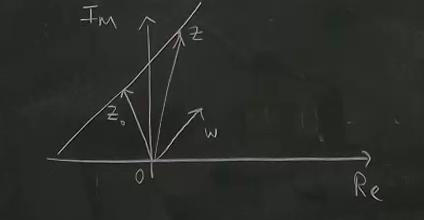
\includegraphics[width=0.5\textwidth]{general_points.png}
% \end{center}
% This is $z = z_0 + \lambda w$ for any $\lambda \in \R$. To eliminate the parameter $\lambda$, take the conjugate
% $$
% \overline{z} = \overline{z_0} + \lambda \overline{w}
% $$
% and combine the equations to get
% $$
% \overline{w} z-w \overline{z}=\overline{w} z_{0}-w \overline{z}_{0}
% $$

% Next, consider the circle with center $c \in \C$ and radius $\rho$.
% \begin{center}
% 	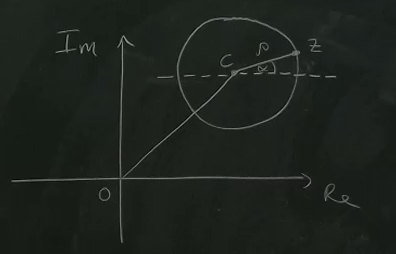
\includegraphics[width=0.5\textwidth]{general_circle.png}
% \end{center}
% A general point on a circle is $z = c + \rho e^{i \alpha}$ for any $\alpha$.
% Equivalently $|z - c| = \rho$. We can even expand this to get
% $$
% |z|^2 - \overline{c} z - c\overline{z} = \rho^2 - |c|^2.
% $$

% \begin{aside}{Aside: Inversion with Complex Numbers}

% We can use \emph{stereographic projection} to understand how inversion works with complex numbers.

% Identify the set $\C_\infty = \C \cup \{\infty\}$ with the Riemann Sphere as shown.
% \begin{center}
% 	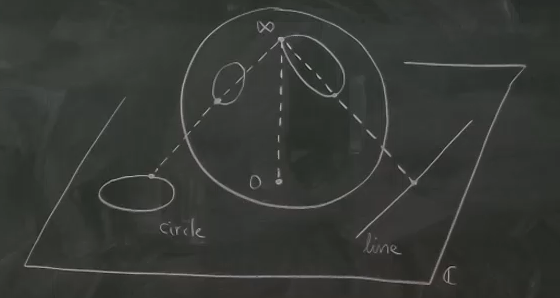
\includegraphics[width=0.5\textwidth]{riemann_sphere.png}
% \end{center}
% Imagine this sphere sitting on the plane at the origin. If we consider points on the sphere, we have a correspondence with points on the plane, created by drawing a line through the north pole (labelled $\infty$) on the sphere through a point on the sphere until it hits the plane (and vice versa). 

% Now when we look at a circle on the complex plane, it will correspond to a circle on the sphere. But also, a line in the plane also corresponds with a circle on the sphere, which goes through the north pole ($\infty$) on the sphere.

% \end{aside}

% \clearpage
% \chapter{Vectors in Three Dimensions}

% What is a vector? The traditional answer to this is that it's a quantity with both magnitude (length, size) and direction.
% There are many examples such quantities: force, momentum, electric and magnetic fields -- but the vector nature of these quantities is essentials the same as the vector notion of position.

% In this section, we will take a geometrical approach to vectors, and we will consider position vectors in 3d space, using standard (Euclidean) notions of points, lines, planes, lengths and angles.

% Chose some point $O$ to be the \vocab{origin}, then points $A, B, \dots$ are represented as displacements from $O$, that is, position vectors, that we write
% $$
% \mathbf{a} = \overrightarrow{OB}, \quad \mathbf{b} = \overrightarrow{OB}, \dots.
% $$

% \begin{center}
% 	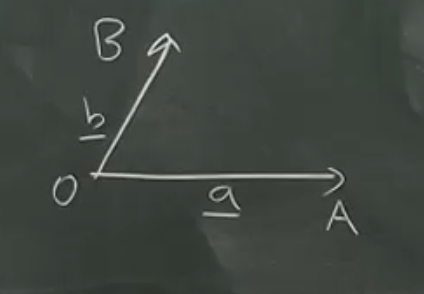
\includegraphics[width=0.3\textwidth]{vector_intro.png}
% \end{center}

% The lengths of these vectors is denoted $|\mathbf{a}| = |\overrightarrow{OA}|$, and we will use $\mathbf{0}$ for the position vector of the origin $O$.

% \section{Vector Addition and Scalar Multiplication}

% We now need to establish what we can do with these vectors: adding them and multiplying them by scalars.

% \begin{definition}[Scalar Multiplication]
% 	Given $\mathbf{a}$, a position vector for some point $A$, and a scalar $\lambda \in \R$, we define $\lambda \mathbf{a}$ to be the position vector of a new point $A'$ on the line $OA$, with $|\lambda \mathbf{a}| = |\lambda||\mathbf{a}|$ and the direction as shown (depending on the sign of $\lambda$).
% 	\begin{center}
% 		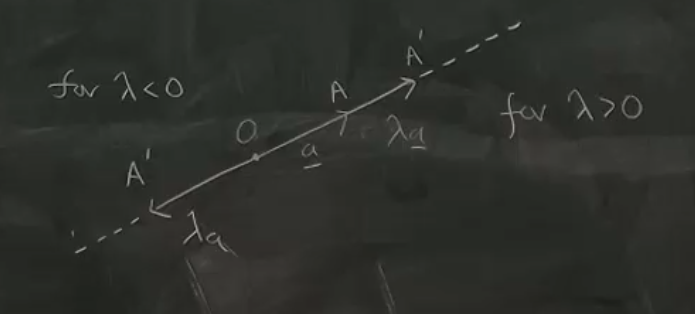
\includegraphics[width=0.5\textwidth]{scalar_multiplication.png}
% 	\end{center}
% \end{definition}

% Using scalar multiplication, we can develop a sensible notion of when two vectors have the same direction, that is, when they are parallel.

% \begin{definition}[Parallelism]
% 	Define $\mathbf{a}$ and $\mathbf{b}$ to be \vocab{parallel}, written $\mathbf{a} \parallel \mathbf{b}$, if and only if
% 	$$
% 	\mathbf{a} = \lambda \mathbf{b} \quad \text{or} \quad \mathbf{b} = \lambda \mathbf{a},
% 	$$
% 	for some $\lambda \in \R$.
% \end{definition}

% In this definition, we allow $\lambda = 0$, so $\mathbf{a} \parallel \mathbf{0}$ for any $\mathbf{a}$. 
% This is slightly non-standard, but is convenient in this course.

% We can also define the addition of vectors.

% \begin{definition}[Vector Addition]
% 	Given $\mathbf{a}, \mathbf{b}$, the position vectors of points $A, B$, if $\mathbf{a} \not\parallel \mathbf{b}$, construct the parallelogram $OACB$. Then define $\mathbf{a} + \mathbf{b} = \mathbf{c}$, the position vector of point $C$ as shown.
% 	\begin{center}
% 		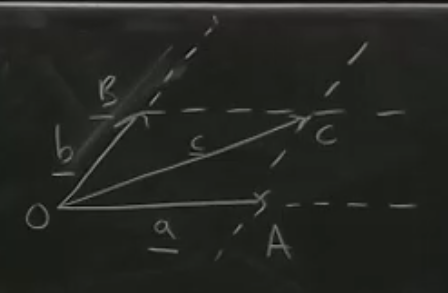
\includegraphics[width=0.45\textwidth]{parallelogram.png}
% 	\end{center} 
% 	If $\mathbf{a} \parallel \mathbf{b}$, then we can write $\mathbf{a} = \alpha \mathbf{u}$ and $\mathbf{b} = \beta \mathbf{u}$ where $\alpha, \beta \in \R$ and $|\mathbf{u}| = 1$. Then $\mathbf{a} + \mathbf{b} = (\alpha + \beta) \mathbf{u}$.
% \end{definition}

% A core idea to vectors is that given any number of them, $\mathbf{a}, \mathbf{b}, \dots, \mathbf{c}$, we can form a \vocab{linear combination}
% $$
% \alpha \mathbf{a} + \beta \mathbf{b} + \cdots + \gamma \mathbf{c},
% $$
% for any $\alpha, \beta, \dots, \gamma \in \R$.

% We can then define the \emph{span} of a linear combination of vectors to be the set of points that can be reached by changing the coefficients.

% \begin{definition}[Span of Multiple Vectors]
% 	We define the \vocab{span} of a set of vectors to be $\operatorname{span} \{\mathbf{a}, \mathbf{b}\} = \{ \alpha \mathbf{a} + \beta \mathbf{b} \; : \; \alpha, \beta \in \R\}$.
% \end{definition}
% If $\mathbf{a} \not \parallel \mathbf{b}$, then this is the plane through points $O$, $A$, $B$.


% We will finish our discussion of vector addition and scalar multiplication by looking at some of the elementary properties that are implied by our definitions.

% \begin{theorem}
% 	Vectors, along with vector addition, form an abelian group.
% \end{theorem}
% \begin{proof}
% 	For any vectors $\mathbf{a}, \mathbf{b}$ and $\mathbf{c}$,\phantom{\qedhere}
% 	\begin{itemize}
% 		\item \emph{Identity}. We have the identity element $\mathbf{0}$, as $\mathbf{a} + \mathbf{0} = \mathbf{0} + \mathbf{a} = \mathbf{a}$.
% 		\item \emph{Inverses}. There exists $-\mathbf{a}$ such that $\mathbf{a} + (-\mathbf{a})= (-\mathbf{a}) + \mathbf{a} = \mathbf{0}$.
% 		\item \emph{Associativity}. $\mathbf{a} + (\mathbf{b} + \mathbf{c}) = (\mathbf{a} + \mathbf{b}) + \mathbf{c}$.
% 		\item \emph{Commutativity}. $\mathbf{a} + \mathbf{b} = \mathbf{b} + \mathbf{a}$. \hfill \qedsymbol
% 	\end{itemize}
% \end{proof}

% \begin{remark}
% 	Given that we defined vector addition geometrically, it is not immediately clear that the associativity holds. Indeed, we really would need to consider the three dimensional construction of a parallelepiped, and check that the construction is indeed associative.
% 	\begin{center}
% 		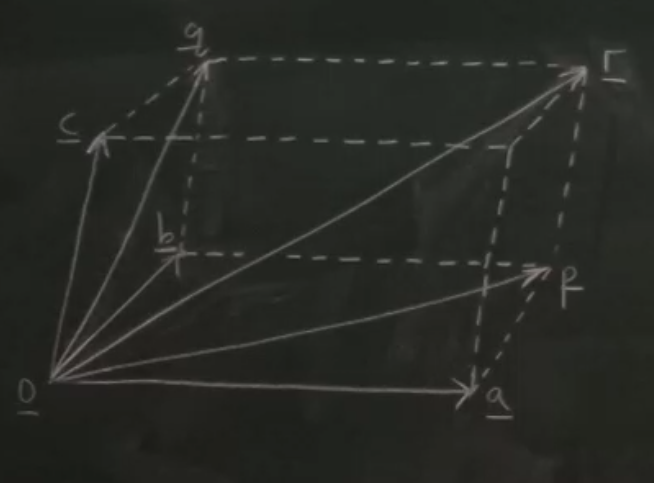
\includegraphics[width=0.5\textwidth]{parallelapiped.png}
% 	\end{center}
% \end{remark}

% \section{The Dot Product}

% This section will involve length and angle in a way that our previous discussion didn't. Although we talked about length, it had more to do with proportionality, and we only touched on angles in regards to vectors being parallel (which is a rather special case).

% \begin{definition}[Dot Product]
% 	Given vectors $\mathbf{a}$ and $\mathbf{b}$, let $\theta$ be the angle between them as shown.
% 	\begin{center}
% 		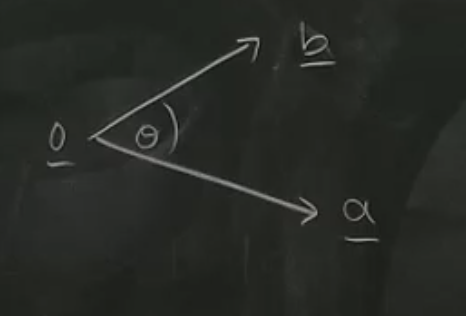
\includegraphics[width=0.4\textwidth]{angle.png}
% 	\end{center}
% 	We define $\mathbf{a} \cdot \mathbf{b} = |\mathbf{a}| |\mathbf{b}| \cos \theta$ to be the \vocab{dot product} of $\mathbf{a}$ and $\mathbf{b}$.  If either of $|\mathbf{a}| = 0$ or $|\mathbf{b}| = 0$, then $\mathbf{a} \cdot \mathbf{b} = 0$.
% \end{definition}

% We can use the dot product to define when two vectors are perpendicular.

% \begin{definition}[Perpendicularity]
% 	We say vectors $\mathbf{a}$ and $\mathbf{b}$ are \vocab{perpendicular} or \vocab{orthogonal}, written $\mathbf{a} \perp \mathbf{b}$, if and only if
% 	$$
% 	\mathbf{a} \cdot \mathbf{b} = 0,
% 	$$
% 	which occurs if and only if $\theta = \pm \pi/2$, when $\theta$ is defined.
% \end{definition}
% As in the definition of parallelism for vectors, we allow $\mathbf{a}$ or $\mathbf{b}$ to be $\mathbf{0}$. This gives us that $\mathbf{0} \perp \mathbf{a}$ for any vector $\mathbf{a}$.


% There is a geometric interpretation of the dot product. For $\mathbf{a}\neq \mathbf{0}$, $|\mathbf{b} | \cos \theta$ is the component of $\mathbf{b}$ along $\mathbf{a}$. We have
% \begin{align*}
% 	|\mathbf{b}| \cos \theta &= \frac{\mathbf{a} \cdot \mathbf{b}}{|\mathbf{a}|} \\
% 	&= \mathbf{u} \cdot \mathbf{b}, \quad \quad \text{where } \mathbf{u} = \frac{\mathbf{a}}{|a|} \text{ is a unit vector along } \mathbf{a} \\
% 	&= | \mathbf{b}_{\parallel} |,
% \end{align*}
% where we resolve the vector $\mathbf{b}$ into parallel and perpendicular components, $\mathbf{b} = \mathbf{b}_{\parallel} + \mathbf{b}_{\perp}$ along $\mathbf{a}$.
% \begin{center}
% 	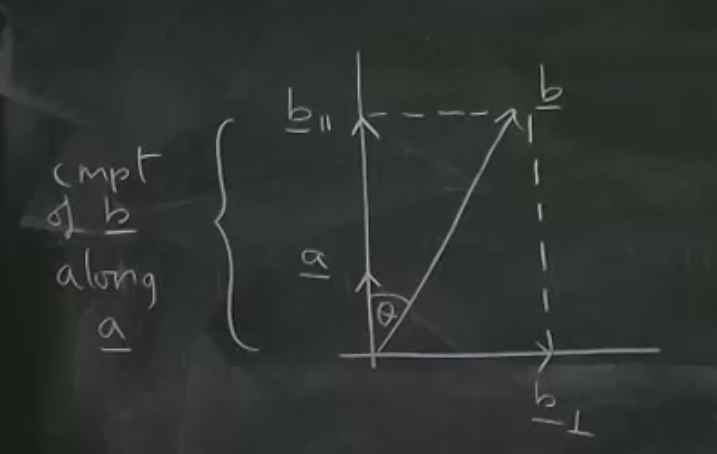
\includegraphics[width=0.4\textwidth]{resolve.png}
% \end{center}
% Note that this implies $\mathbf{a} \cdot \mathbf{b} = \mathbf{a} \cdot \mathbf{b}_{\parallel}$.

% We now state some elementary properties of the dot product.

% \begin{proposition}[Properties of the Dot Product]
% 	Let $\mathbf{a}$ and $\mathbf{b}$ be vectors, and $\lambda \in \R$.
% 	\begin{enumerate}[label=(\roman*)]
% 		\item $\mathbf{a} \cdot \mathbf{b} = \mathbf{b} \cdot \mathbf{a}$.
% 		\item $\mathbf{a} \cdot \mathbf{a} = |\mathbf{a}|^2 \geq 0$, with equality if and only if $\mathbf{a} = \mathbf{0}$.
% 		\item $(\lambda \mathbf{a}) \cdot \mathbf{b} = \lambda ( \mathbf{a} \cdot \mathbf{b}) = \mathbf{a} \cdot (\lambda \mathbf{b})$.
% 		\item $\mathbf{a} \cdot (\mathbf{b} + \mathbf{c}) = \mathbf{a} \cdot \mathbf{b} + \mathbf{a} \cdot \mathbf{c}$.
% 	\end{enumerate}
% \end{proposition}
% \begin{proof}[Proof Sketch]
% 	These all follow immediately from the definition of the dot product.
% \end{proof}

% \section{The Cross Product}

% The dot product is an operation that takes two vectors and gives us back a real number. We will now define an operation that takes two vectors and returns another vector, that has a specific spacial relationship with the two given vectors. It is important to note that what we define in this section will only hold for three dimensional vectors.

% \begin{definition}[Cross Product]
% 	Given vectors $\mathbf{a}$ and $\mathbf{b}$, let $\theta$ be the angle between them, measured as shown, with respect to a  unit vector $\mathbf{n}$ which is normal (perpendicular) to the plane spanned by the two vectors.
% \begin{center}
% 	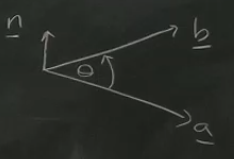
\includegraphics[width=0.3\textwidth]{cross-product-angle.png}
% \end{center}
% we define $\mathbf{a} \times \mathbf{b} = |\mathbf{a} | |\mathbf{b}| \sin \theta \mathbf{n}$ to be the \vocab{cross product} of $\mathbf{a}$ and $\mathbf{b}$.
% \end{definition}

% \begin{remark}
% 	The normal vector $\mathbf{n}$ is defined up to a sign $\pm 1$ if $\mathbf{a} \not \parallel \mathbf{b}$, but changing the sign of $\mathbf{n}$ changes the angle $\theta$ to $2 \pi - \theta$, and $\mathbf{a} \times \mathbf{b}$ is unchanged. If $\mathbf{a} \parallel \mathbf{b}$, then $\mathbf{n}$ is not defined, but then $\theta = 0$ or $|\mathbf{a}|$ or $|\mathbf{b}| = 0$. But $\mathbf{a} \times \mathbf{b} = \mathbf{0}$ in these cases.
% \end{remark}

% As there was for the dot product, there is a geometric interpretation of the cross product.
% For vectors $\mathbf{a}$ and $\mathbf{b}$, the magnitude of their cross product, $|\mathbf{a} \times \mathbf{b}|$ is the area of the parallelogram shown below.
% \begin{center}
% 	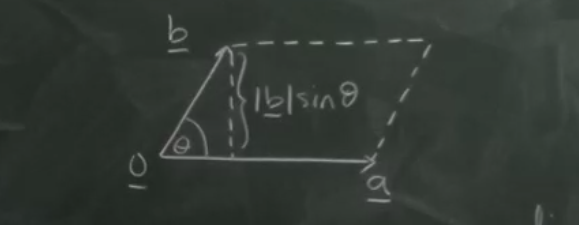
\includegraphics[width=0.4\textwidth]{cross_product_area.png}
% \end{center}
% $$
% |\mathbf{a} \times \mathbf{b} = |\mathbf{a}| |\mathbf{b}| \sin \theta = (\text{base})\times(\text{height}) = \text{area}.
% $$

% Finally, we will at the elementary properties of the cross product.

% \begin{proposition}[Properties of the Cross Product]
% 	Let $\mathbf{a}$ and $\mathbf{b}$ be vectors, and $\lambda \in \R$.
% 	\begin{enumerate}[label=(\roman*)]
% 		\item $\mathbf{a} \times \mathbf{b} = - \mathbf{b} \times \mathbf{a}$.
% 		\item $(\lambda \mathbf{a}) \times \mathbf{b} = \lambda(\mathbf{a} \times \mathbf{b}) = \mathbf{a} \times (\lambda \mathbf{b})$.
% 		\item $\mathbf{a} \times (\mathbf{b} + \mathbf{c}) = \mathbf{a} \times \mathbf{b} + \mathbf{a} \times \mathbf{c}$.
% 		\item $\mathbf{a} \times \mathbf{b} = \mathbf{0}$ if and only if $\mathbf{a} \parallel \mathbf{b}$.
% 		\item $(\mathbf{a} \times \mathbf{b}) \perp \mathbf{a}$ and $)\mathbf{a} \times \mathbf{b}) \perp \mathbf{b}$.
% 	\end{enumerate}
% \end{proposition}
% \begin{proof}[Proof Sketch]
% 	These follow directly from the definition of the cross product.
% \end{proof}

% \section{Orthonormal Basis \& Components}

% We can use the geometrical approach developed previously to describe vectors.
% We begin by choosing vectors
% $$
% \mathbf{e}_1,\  \mathbf{e}_2,\  \mathbf{e}_3
% $$
% that are \emph{orthonormal}.

% \begin{definition}[Orthonormal]
% 	We say two vectors $\mathbf{u}$ and $\mathbf{v}$ are \vocab{orthonormal} if they are of unit length and are orthogonal (perpendicular) to each other.
% \end{definition}

% So in this case, we have to have
% $$
% \mathbf{e}_i \cdot \mathbf{e}_j = \begin{cases}
% 	1 & \mbox{if } i = j \\
% 	0 &\mbox{if } i \neq j
%    \end{cases} 
% $$
% Choosing these vectors is equivalent to choosing a cartesian axis, along the directions of the vectors. These vectors form a \emph{basis}.\footnote{We will define a basis only for the case of three dimensional vectors for the time being.}

% \begin{definition}[Basis]
% 	We say that some set of vectors $\{\mathbf{e}_1, \mathbf{e}_2, \mathbf{e}_3\}$ is a \vocab{basis} if any vector can be written as
% 	$$
% 	\mathbf{a} = \sum_{i = 1}^3 a_i \mathbf{e}_i = a_1 \mathbf{e}_1 + a_2 \mathbf{e}_2 + a_3 \mathbf{e}_3,
% 	$$
% 	where each \vocab{component} $a_i$ is uniquely determined by $a_i = \mathbf{e}_i \cdot \mathbf{a}$.
% \end{definition}
% \begin{center}
% 	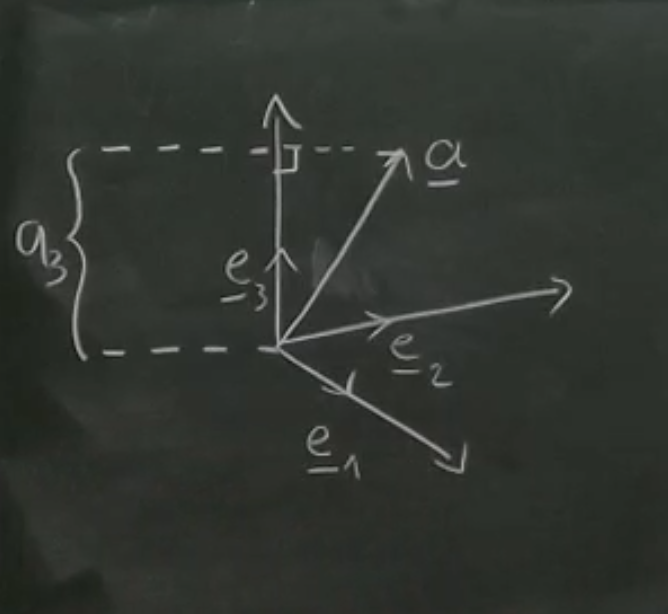
\includegraphics[width=0.25\textwidth]{basis.png}
% \end{center}

% Once this is done, we can think of vectors as sets of numbers, that is, we identify a vector $\mathbf{a}$ with it's components, writing it as
% $$
% \mathbf{a} = \begin{pmatrix}
% 	a_1 & a_2 & a_3
% \end{pmatrix},
% $$
% which is a \vocab{row vector}, or as
% $$
% \mathbf{a} = \begin{pmatrix}
% 	a_1 \\ a_2 \\ a_3
% \end{pmatrix},
% $$
% which is a \vocab{column vector}.
% With this representation, we can see what the dot and cross product look like.
% \begin{align*}
% 	\mathbf{a} \cdot \mathbf{b} &= (a_1 \mathbf{e}_1 + a_2 \mathbf{e}_2 + a_3 \mathbf{e}_3) \cdot (b_1 \mathbf{e}_1 + b_2 \mathbf{e}_2 + b_3 \mathbf{e}_3)\\
% 	&= a_1 b_1 + a_2 b_2 + a_3 b_3.
% \end{align*}
% We also get
% $$
% |\mathbf{a}|^2 = \mathbf{a} \cdot \mathbf{a} = a_1^2 + a_2 ^2 + a_3^3,
% $$
% which is equivalent to the pythagorean theorem.
% For the cross product, we first need to establish the cross products between the basis vectors.
% We know that $\mathbf{e}_1 \times \mathbf{e}_2$ is going to be of unit length, and perpendicular to both $\mathbf{e}_1$ and $\mathbf{e}_2$, but that doesn't estabish if it will point in the direction of $\mathbf{e}_3$ or $-\mathbf{e}_3$.


\end{document}